\chapter{Programmazione Lineare}

\section{Cosa è la programmazione lineare?}
\subsection{Definizione}
La programmazione lineare è quella branca della ricerca operativa che si occupa di studiare algoritmi di risoluzione per problemi di ottimizzazione lineare.

\subsection{Utilizzo comune}
Il più comune tipo di applicazione della programmazione lineare riguarda il problema generale della allocazione di risorse limitate tra attività concorrenti nel modo migliore possibile.

\subsection{Perchè "lineare"?}
La programmazione lineare utilizza un modello matematico per descrivere il problema in esame.
L'aggettivo lineare indica che \uline{tutte le funzioni matematiche del modello devono essere \textbf{funzioni lineari}}.

La parola programmazione non si riferisce, in questo caso, a quella dei computer ma è, piuttosto un sinonimo per pianificazione.

\subsection{Obiettivo}
La programmazione lineare riguarda, quindi, la pianificazione delle attività al fine di ottenere un risultato ottimilae, coiè il raggiungimento dell'obiettivo prefissato nella maniera migliore tra le possibili alternative


\newpage
\section{Formulazione di un problema}
\subsection{Funzione obiettivo}
\begin{minipage}{0.45\textwidth}
    {
        \Large
    
        $$
            \operatorname*{opt}_{\mathbf{x} \in X} Z = \sum_{j=1}^{n} c_j \cdot x_j
        $$
    }
\end{minipage}
\hfil
\begin{minipage}{0.45\textwidth}
    Funzione obiettivo $Z$ con $n$ numero di variabili decisionali
    \begin{itemize}
        \item $\mathbf{c_j}$: Coefficienti di costo
        \item $\mathbf{x_j}$: Variabili decisionali
    \end{itemize}
\end{minipage}

\subsection{Vincoli del problmea di ottimizzazione}
\begin{minipage}{0.45\textwidth}
{
    \Large

    $$
        \sum_{j=1}^{n} a_{ij} \cdot x_j \leq b_i \ i=1,\dots,m
    $$
}
\end{minipage}
\hfil
\begin{minipage}{0.45\textwidth}
    Vincoli che definiscono la regione ammissibile $X$ con $m$ numero di vincoli

    \begin{itemize}
        \item $\mathbf{a_{ij}}$: Termini noti sinistri
        \item $\mathbf{x_j}$: Variabili decisionali
        \item $\mathbf{b_i}$: Termini noti destri
    \end{itemize}
\end{minipage}

\section{Assunzioni}
Un problema di programmazione lineare si poggia sulle seguenti \textbf{assunzioni implicite}

\subsection{Assunzione di Proporzionalità}
\subsubsection{Definizione semplificata}
Il contributo di ogni variabile decisionale, al valore della funzione obiettivo, è proporzionale rispetto al valore assunto dalla variabile stessa

\subsubsection{Definizione matematica}
Il contributo di ogni attività al valore della \textbf{funzione obiettivo} $\mathbf{Z}$ è proporzionale al \textbf{livello dell'attività} $x_j$ secondo 

$$
    Z = \sum_{j=1}^{n} c_j \cdot x_j
$$

Analogamente, il contributo di ogni attività al \textbf{vincolo} $\mathbf{"i"}$ è proporzionale al livello di attività $x_j$ secondo

$$
    \sum_{j=1}^{n} a_{ij} \cdot x_j \leq b_i
$$

\subsubsection{Esempio 1}
\begin{minipage}[t]{0.45\textwidth}
    \vspace{0pt}

    I due punti sulla retta, $(1, 3)$ e $(2, 6)$, mostrano che al raddoppiare della variabile $x_1$ (da 1 a 2), anche il valore della funzione obiettivo sull'asse verticale $Z$ raddoppia (da 3 a 6). 
    
    Questo illustra il vincolo di proporzionalità tipico della programmazione lineare: il contributo di ogni variabile alla funzione obiettivo è direttamente proporzionale al valore della variabile stessa.
\end{minipage}
\hfill
\begin{minipage}[t]{0.45\textwidth}
    \vspace{0pt}
    \begin{center}
            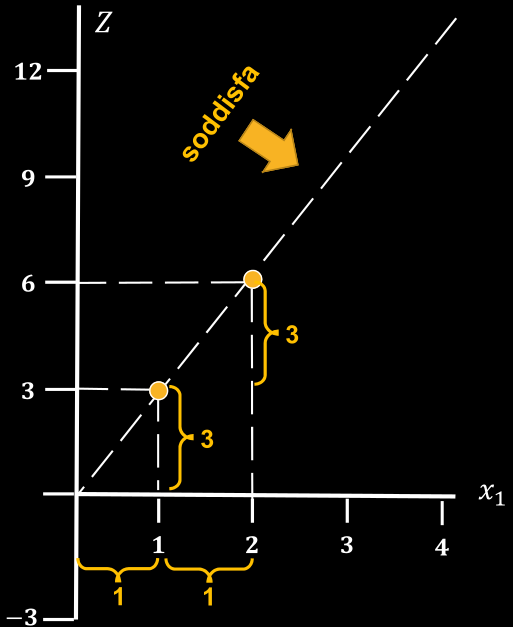
\includegraphics[scale=0.5]{Immagini/Proporzionalità1.png}
    \end{center}
\end{minipage}

\subsubsection{Esempio 2}
\begin{minipage}[t]{0.45\textwidth}
    L'immagine a destra mostra una situazione simile ma con un "costo di inizializzazione" (l'intercetta a $-1$ sull'asse verticale). 
    
    Questo introduce un elemento non lineare (affine, più precisamente), poiché il rapporto tra l'incremento di $Z$ e l'incremento di $x_1$ non è più costante rispetto all'origine. 
\end{minipage}
\hfill
\begin{minipage}[t]{0.45\textwidth}
    \vspace{0pt}
    \begin{center}
        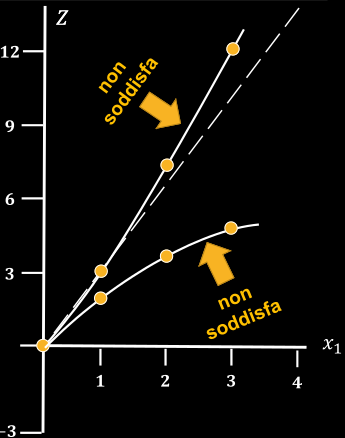
\includegraphics[scale=0.75]{Immagini/Proporzionalità 2.png}
    \end{center}
\end{minipage}

\newpage
\subsection{Assunzione di Additività}
\subsubsection{Definizione semplificata}
Ogni funzione è la somma dei contributi delle variabili decisionali

\subsubsection{Definizione matematica}
In un problema di programmazione lineare, il valore assunto da ogni funzione, sia essa \textbf{funzione obiettivo} o vincolo, è dato dalla somma dei contributi individuali delle rispettive attività

\subsubsection{Esempio}
\begin{center}
    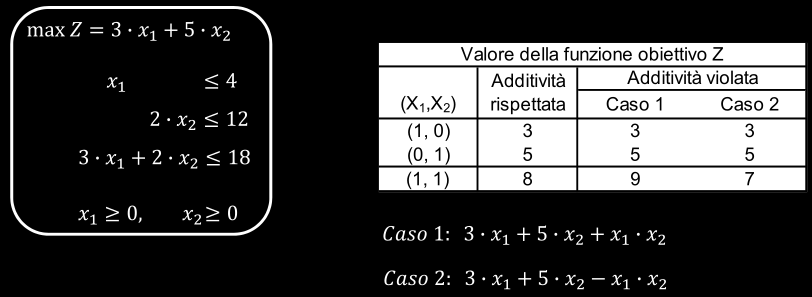
\includegraphics[scale=0.65]{Immagini/Additività.png}
\end{center}

\subsection{Assunzione di Divisibilità}
Le variabili decisionali in un programma di programmazione lineare sono libere di assumere qualsiasi valore, inclusi valori non interi che soddisfino i vincoli funzionali ed i vincoli di non negatività ( in altri termini, le variabili continue).

In alcune condizioni può accadere che le variabili decisionali non possano che assumere valori interi (non è possibile costruire un quarto di finiestra, non è possibile produrre 21.45 porte finestra).

In questi casi si parla di problema di programmazione lineare intera o a numeri interi

\subsection{Assunzione di Certezza}
Il valore assegnato ad ogni parametro di un problema di programmazione lineare è assunto essere non con certezza e costante

\newpage
\section{Soluzione Grafica}
\subsection{Cosa è?}
Per risolvere i problemi di programmazione lineare, possiamo adottare una procedura grafica, determinando i valori delle variabili decisionali $x_1,x_2$ che rispettano i vincoli, ed al tempo stesso rendendo massimo il valore $Z$ della funzione obiettivo.

La soluzione grafica si compone di:
\begin{itemize}
    \item Disegno della regione ammissibile
    \item Determinazione dell'ottimo
\end{itemize}

\subsection{Vincoli di Uguaglianza}
I vincoli $g_i(x)$ possono essere:
\begin{itemize}
    \item \textbf{Rette:} $g_i(x)=0$
    
    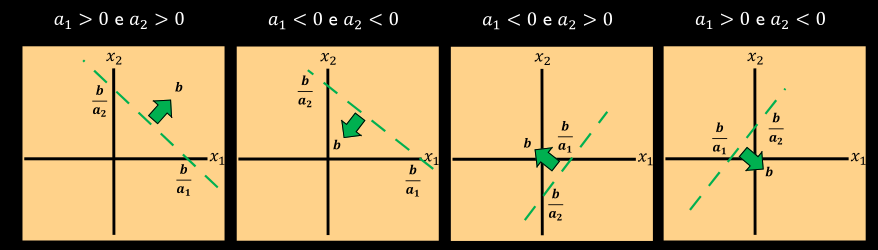
\includegraphics[scale=0.5]{Immagini/Rette.png}

    \item \textbf{Semipiani:} $g_i(x) \leq 0$
\end{itemize}

\subsubsection{Come rappresentiamo un semipiano?}
\begin{enumerate}
    \item Disegnamo la retta associata $(a_1 \cdot x_1 + a_2 \cdot x_2 \leq b)$
    \item Scegliamo un punto non appartenente a tale retta
    \begin{itemize}
        \item Se il punto verifica la disuguaglianza allora scegliamo il semipiano che lo contiene
        \item Altrimenti scegliamo l'altro semipiano
    \end{itemize}
\end{enumerate}

\begin{center}
    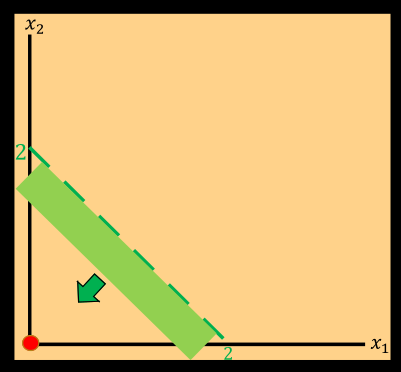
\includegraphics[scale=0.5]{Immagini/Semipiano.png}
\end{center}

\newpage
\subsection{Vincoli funzionali di $\leq$}
In maniera generalizzata, possiamo pensare che un problema di programmazione lineare è formulato in questo modo:

\begin{center}
    \[
    \setlength{\arraycolsep}{3pt}
    \begin{array}{l c c c c c c c l}
        \max Z = & c_1 \cdot x_1 & + & c_2 \cdot x_2 & + & \dots & + & c_n \cdot x_n & \\
        [1.5ex]
        & a_{11} \cdot x_1 & + & a_{12} \cdot x_2 & + & \dots & + & a_{1n} \cdot x_n & \leq b_1 \\
        [1ex]
        & a_{21} \cdot x_1 & + & a_{22} \cdot x_2 & + & \dots & + & a_{2n} \cdot x_n & \leq b_2 \\
        [1ex]
        & \dots \dots & + & \dots \dots & + & \dots & + & \dots \dots & \leq \dots \\
        [1ex]
        & a_{m1} \cdot x_1 & + & a_{m2} \cdot x_2 & + & \dots & + & a_{mn} \cdot x_n & \leq b_m \\
        [1.5ex]
        & \multicolumn{8}{l}{x_1 \geq 0, x_2 \geq 0, \dots, x_n \geq 0}
    \end{array}
    \]
\end{center}

Con :
\begin{itemize}
    \item Z funzione obiettivo
    \item $
    % \left. crea una delimitazione sinistra invisibile
    \left.
    \setlength{\arraycolsep}{3pt}
    \begin{array}{c c c c c c c l}
        a_{11} \cdot x_1 & + & a_{12} \cdot x_2 & + & \dots & + & a_{1n} \cdot x_n & \leq b_1 \\
        [1ex]
        a_{21} \cdot x_1 & + & a_{22} \cdot x_2 & + & \dots & + & a_{2n} \cdot x_n & \leq b_2 \\
        [1ex]
        \dots\dots & + & \dots\dots & + & \dots & + & \dots\dots & \leq \dots \\
        [1ex]
        a_{m1} \cdot x_1 & + & a_{m2} \cdot x_2 & + & \dots & + & a_{mn} \cdot x_n & \leq b_m 
    \end{array}
    % \right\} chiude il blocco con una graffa destra che si adatta all'altezza
    \right\} \text{ Vincoli funzionali}
    $
    \item $x_1 \geq 0,\ x_2\geq 0,\ x_3 \geq 0,\ \dots,\ x_m\geq 0$ vincoli di non negatività 
\end{itemize}

In particolare quindi:
\begin{itemize}
    \item $\mathbf{Z}$: Valore della misura di prestazione
    \item $\mathbf{x_j}$: Livello dell'attività $j$
    \item $\mathbf{c_j}$: Incremento del valore della misura di prestazione $Z$ corrispondente all'incremento di un'unità del valore dell'attività $x_j$
    \item $b_i$: Quantità di risorsa $"i"$ allocabile all'attività $x_j,\ j=1,\ \dots,\ n$
    \item $a_{ij}$: Quantità di risorsa $"i"$ consumata da ogni unitò di attività $x_j\ j=1,\ \dots,\ n$
\end{itemize}

\subsection{Vincoli di funzionalità di $\geq$ e $=$}
Generalizzando al caso con $n$ \textbf{variabili decisionali} ed $m$ \textbf{vincoli}, otteniamo la seguente formulazione di un \textbf{programmazione lineare}

\begin{itemize}
    \item \textbf{Funzione obiettivo:}: $opt\ Z$
    \item \textbf{Vincoli}: 
    $
    % \left. crea una delimitazione sinistra invisibile
    \left.
    \setlength{\arraycolsep}{3pt}
    \begin{array}{c c c c c c c l}
        a_{11} \cdot x_1 & + & a_{12} \cdot x_2 & + & \dots & + & a_{1n} \cdot x_n & \leq b_1 \\
        [1ex]
        a_{21} \cdot x_1 & + & a_{22} \cdot x_2 & + & \dots & + & a_{2n} \cdot x_n & \leq b_2 \\
        [1ex]
        \dots\dots & + & \dots\dots & + & \dots & + & \dots\dots & \leq \dots \\
        [1ex]
        a_{m1} \cdot x_1 & + & a_{m2} \cdot x_2 & + & \dots & + & a_{mn} \cdot x_n & \leq b_m 
    \end{array}
    % \right\} chiude il blocco con una graffa destra che si adatta all'altezza
    \right\} \text{ Vincoli funzionali}
    $
\end{itemize}

In questo caso quindi, siamo nel caso quale $x_2$ \textbf{non è vincolata} da nessun valore.

Inoltre, ogni vincolo $\geq$ e $=$ può essere riscritto nella seguente forma

\begin{itemize}
    \item $g_i(x) \geq b_i \to -g_i(x) \leq b_i$
    \item $g_i(x) = b_i \to 
    \begin{cases}
        g_i(x) \geq b_i \\
        g_i(x) \leq b_i    
    \end{cases}$
\end{itemize}

\section{Regione Ammissibile}
\subsection{Definizione}
La regione ammissibile $X$ è data dal soddisfacimento dei vari vincoli

$$
X = \{x \in \mathbb{R}^n : g_i(x) =   \left\{
        \begin{matrix}
        \geq \\
        = \\
        \leq
        \end{matrix}
        \right\}0,\ i=1,\ \dots,\ m
    \}
    \text{ con } g_i(x)=a_i^T-b_i
$$

dove $a \in \mathbb{R}^n. b\in\mathbb{R}^m$

\subsection{Proprietà della Regione Ammissibile}
La regione ammissibile, da un punto di vista geometrico, corrisponde ad un \textbf{poliedro convesso in } $\mathbf{R}^n$.

La regione ammissibile può essere limitata o illimitata

\begin{center}
    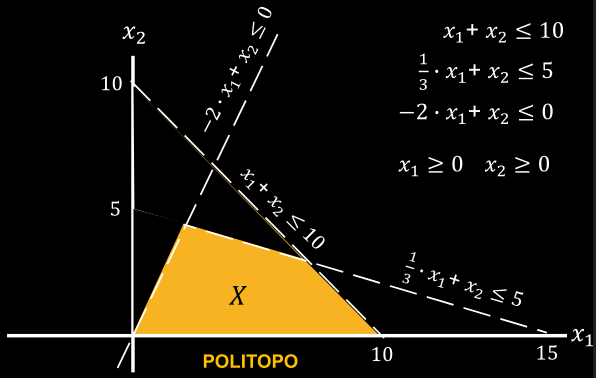
\includegraphics[scale=0.5]{Immagini/RA PL.png}
\end{center}

\subsection{Possibili soluzioni}
Si possono verificare 4 soluzioni:
\begin{itemize}
    \item Il problema di programmazione lineare \textbf{ammette una sola soluzione ottima in un vertice del poligono convesso} che delimita la regione ammissibile
    \item Il problema di programmazione lineare \textbf{ammette infinite soluzioni ottime in un lato del poligono commesso} che delimita la regione ammissibile se la direzione di decrescita è perpendicolare ad un lato del poligono
    \item Il problema di programmazione lineare \textbf{ammette infinite soluzioni} perchè la regione ammissibile è illimitata e la funzione obiettivo è illimitata superiormente (se è di massimizzazione) o inferiormente (se di minimizzazione)
    \item Il problema di programmazione \textbf{non ammette soluzione} perchè la regione ammissibile è vuota 
\end{itemize}

Per risolvere quindi un problema di programmazione lineare:
\begin{enumerate}
    \item Disegnare la regione ammissibile
    \item Cercare di massimizzare/minizzare la soluzione, riportando ciò che troviamo sul grafico
\end{enumerate}
